\documentclass[main.tex]{subfiles}
\begin{document}
\chapter{Background}\label{chap:Background}
In this chapter, we will present relevant literature needed to completely understand the proposed concept of \autoref{chap:Concept}.


\section{Intel Realsense}
% TODO datasheet der D455 und T256 hier rein pasten.
\href{https://www.intelrealsense.com/compare-depth-cameras/}{https://www.intelrealsense.com/compare-depth-cameras/}

\subsection*{SLAM}
SLAM (Simultaneous Localization And Mapping) algorithms aim to solve a usual problem in the field of unmanned robotics;
A robot finds itself in an unknown environment and attempts to build a coherent map while keeping track of its location.
Over decades of research on this particular problem, many different methodologies have been developed, usually regarding the sensors used to aid the robot's navigation.
Since odometry sensors like rotary encoders that measure the rotation of the robot's wheels are unreliable when it comes to uneven or slippery ground, visual sensors also needed to be involved.

\paragraph*{RTAB-MAP}
RealSense-ROS internally uses a SLAM algorithm for map building, namely RTAB-MAP (Real-Time Appearance-Based Mapping)\cite{Labbé_Michaud_2019}.
Unlike purely visual-based SLAM algorithms, RTAB-MAP also takes input from odometry sensors, as well as an optional additional input in form of two- or three-dimensional 
lidar scan.
All these inputs are combined during a synchronization step, the results of which are passed to RTAB-MAP's \textit{Short-Term-Memory} (STM).
The STM assembles a new node from the new inputs and inserts it into the map graph. Based on the newly inserted node, a loop closure is calculated.
If a loop closure is detected, the map graph is optimized and thus minimized. In addition, the global map is reassembled in correspondence with the new information.
The resulting map is published in form of an unorganized point cloud.

RTAB-MAP's general workflow is depicted in Figure~\ref{fig:rtabmap}:
\begin{figure}[!h]
    \centering
    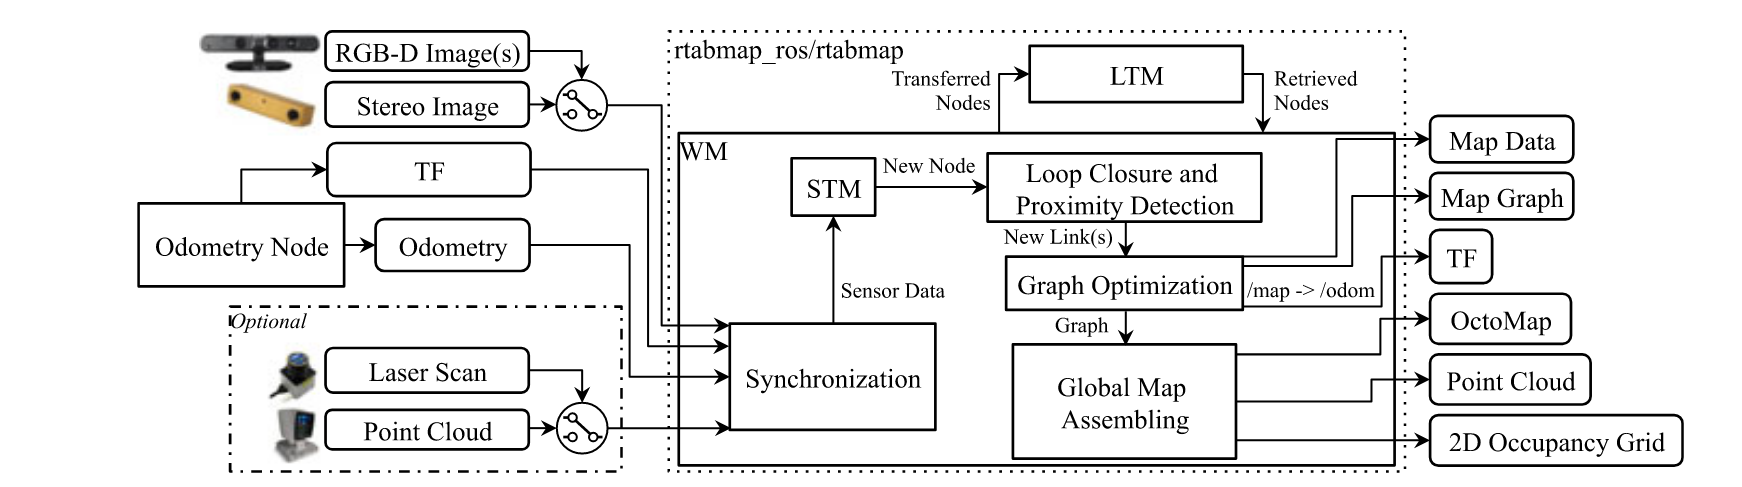
\includegraphics[width=15 cm]{images/rtabmap.png}
    \caption{Block diagram of RTAB-MAP's main node. Taken from \cite[Figure~1]{Labbé_Michaud_2019}}
    \label{fig:rtabmap}
\end{figure}

\section{Plane Detection}

\paragraph*{introduction}
The field of plane detection has been around for decades. Most methods of detecting planar regions can be sorted into one of three main categories:
\begin{itemize}
    \item Hough Transform (HT)
    \item RANSAC (RC)
    \item Region Growing (RG)
\end{itemize}

\subsection*{Hough Transform}
HT wurde ursprünglich introduced um lines in bildern zu finden. das ganze wurde aber inzwischen erweitert auf weitere 
formen im zwei und sogar drei dimensionalen raum.
Möchte man in 2d punktdaten eine gerade detektieren, legt man durch jeden datenpunkt für jede orientierung eine gerade in hesse normal form. Dabei werden stimmen für 
die winkel abgegeben, welche ähnliche distanzen zum ursprung erzeugen. Am ende hat die best fitting grade den winkel, für den die meisten punkte gestimmt haben.
Die datenstruktur, in dem die Stimmen gesammelt werden, wird auch accumulator genannt.


\subsection*{RANSAC}
RANSAC (RAndom SAmple Consensus) has been researched for decades. While many use cases revolve around image processing, it is also heavily employed in many plane detection algorithms\cite{Sun_Mordohai_2019,Yang_Forstner,Ashraf_Ahmed_2017}.
RANSAC is an iterative process. Each iteration randomly samples a certain amount of data points and fits a mathematical model through them. The level of outliers determines the quality of the obtained model and preserves the best overall model.
In the context of this work, the model parameters would be some plane equation or a combination of normal vectors and center points.

\subsection*{Region Growing}
Region Growing methods are often used in the field of image or point cloud segmentation \cite{Proença_Gao_2018, Vo_Truong-Hong_Laefer_Bertolotto_2015}. 
RG-based segmentation methods aim to obtain a set of disjoint regions by initially selecting a set of seed points and incrementally inserting neighboring points based on an inclusion criterion. 
Therein, the quality of results depends on the choice of seed points, e.g., a very noisy seed point could decrease overall quality  \cite{Malek_Rahman_Yasiran_Jumaat_Jalil_2012}.   
In the context of this work, a criterion for region growth could be the distance or curvature between a region and its adjacent data points. 

\section{Plane Detection Algorithms}
In dieser section werden die algorithmen näher erläutert, die im späteren kontext dieser arbeit im fokus stehen werden.

\subsection{RSPD}
RSPD (Robust Statistics approach for Plane Detection \cite{Araújo_Oliveira_2020}) is based on region growing. After taking an unorganized point cloud as input, the procedure is divided into three phases; 
\textit{Split, Grow and Merge}.

\paragraph*{Split}
The authors use an octree to recursively subdivide the point cloud. The subdivision is repeated until every leaf node contains less than $0.1\%$ of the total amount
of points.
This is followed by a planarity test, during which the octree is traversed bottom-up. If all eight children of a node $n$ are leaf nodes and fail the planarity test, $n$ replaces its children
by becoming a leaf node of its own. This procedure is repeated until the root of the octree is reached.
 
\paragraph*{Grow}
In preparation for the growth phase, a neighborhood graph (NG) over the entire point cloud is created. Every node of NG represents one point and an edge between two nodes exists only if
a k-nearest-neighbor search detects both points being in the same neighborhood. 

The graph construction is subsequently followed by a breadth-first-search, during which a point $x$ is inserted into a planar patch $p$ if it satisfies the following conditions:
\begin{itemize}
    \item $x$ is not included in any patch
    \item $x$ satisfies the inlier conditions for $p$ % TODO prob explain them right
\end{itemize}

\paragraph*{Merge}
In the last phase, the previously grown patches are merged. Two planar patches $P_1$ and $P_2$ can be merged, if the following conditions are met: 
\begin{itemize}
    \item the octree nodes of $P_1$ and $P_2$ are adjacent
    \item $P_1.n$ and $P_2.n$ have a divergence within a tolerance range
    \item at least one inlier of $P_1$ satisfies the inlier condition from $P_2$ and vice versa
\end{itemize}

This phase returns all maximally merged planar patches, i.e. the final planes.

\subsection{OPS}
OPS (Oriented Point Sampling for plane detection \cite{Sun_Mordohai_2019}) accepts an unorganized point cloud as input.
First, a sample of points is uniformly selected. The normal vectors of these points are estimated using SVD and the k nearest neighbors, which had been obtained by the use of a k-d tree.
An inverse distance weight function is employed to prioritize neighboring points that are closer to the sample of which the normal vector is currently being estimated.


After normal estimation, one-point-RANSAC is used to find the largest plane. Usual RANSAC implementations sample three points to fit a plane, however, OPS fits a plane with only one sample point and its normal vector.
Once a plane with the most inliers is obtained, its normal vector is re-estimated using SVD on all inliers and all inliers are removed from the point cloud.
This process is repeated until the number of remaining points falls below a predefined threshold $\theta_N$.

\subsection{3D-KHT}\label{sub:3dkht}
\citeauthor{Limberger_Oliveira_2015} propose a hough transform-based plane detection method, which accepts unorganized point clouds as input \cite{Limberger_Oliveira_2015}.
The point cloud is spatially subdivided. The authors propose the usage of octrees over k-d trees because the k-d tree lacks efficiency in terms of 
creation and manipulation. Furthermore, the octree succeeds in capturing the shapes inside the point cloud, while the k-d tree does not.   

Using the octree, the point cloud is subdivided until either the points inside a leaf node are considered approximately coplanar or the number of points is less than 
a predefined threshold. The authors recommend this threshold to value 30 for large point clouds.
The approximately coplanar nodes are refined by removing outliers and subsequently fitting a plane through the remaining points.

% kernel calculation + cluster voting

In dieser Phase werden zuerst gaussische trivariate kernel berechnet. Dabei wird die Ebene in spherical coordinates umgeschrieben.
% TODO rest of 3dkht, explain hough transform first
\textcolor{red}{hier noch den rest einfügen!}

\subsection{OBRG} \label{sec:bg-obrg}
OBRG (Octree-Based Region Growing \cite{Vo_Truong-Hong_Laefer_Bertolotto_2015}) is also a method that employs region growing.

First, an unorganized point cloud is recursively subdivided using an octree. 
An octree node $n$ repeatedly subdivides itself into eight children until the level of $n$ superseded a predefined maximum subdivision value or if the
amount of contained points in $n$ is less than a predefined minimum of included points.  

Saliency features are calculated for every leaf node in preparation for the region growing step. A normal vector is obtained by performing a principle 
component analysis (PCA) on the points inside each leaf node. The best-fitting plane of each leaf is defined by the normal vector and its center point.
A residual value is obtained by taking the RMS of the distance of all included points to the plane.

All leaf nodes are selected as individual seed points. Starting from the seed with the lowest residual value, which relates to a low amount of noise, 
a neighboring leaf node $n$ is inserted into the region if $n$ does not belong to any region and the angular divergence between both normal vectors is smaller than 
a predefined threshold. 

Lastly, a refinement step is employed. 
Fast refinement (FR) is performed on regions that succeed in a planarity test (70\%-90\% of included points fit the best plane). FR is leaf-based, and all previously unallocated neighboring nodes that satisfy an inlier criterion are added to the region.
General refinement (GR) is performed on regions that are considered non-planar. In contrast to the fast refinement, GR is point based. Therefore, 
points from neighboring and previously unallocated leaf nodes are considered and inserted into the region if they, too, satisfy the inlier criterion.
The refinement process returns a complete set of planar regions. 

\end{document}



